62. \begin{figure}[ht!]
\center{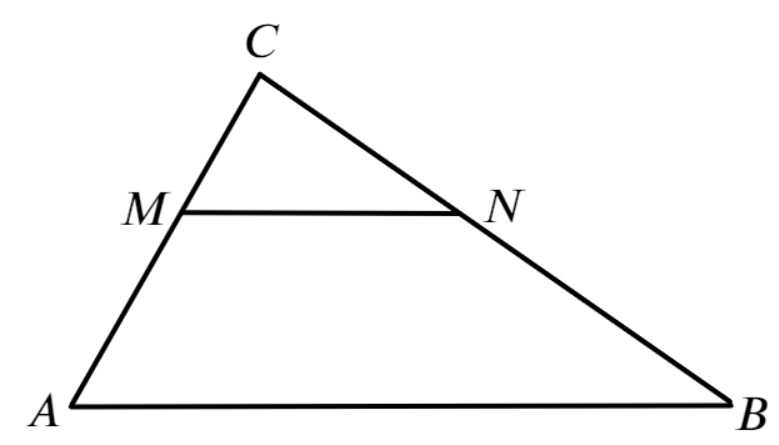
\includegraphics[scale=0.35]{g8-62.png}}
\end{figure}\\
Треугольники $MCN$ и $ABC$ подобны по двум углам (общий и соответственные при паралелльных прямых $MN$ и $AB$), коэффициент подобия равен $\cfrac{2}{3+2}=\cfrac{2}{5}.$ Тогда если $S_{\Delta ABC}=S,$ то $S_{\Delta MCN}=\cfrac{4}{25}S,$ а $S_{AMNB}=S-\cfrac{4}{25}S=\cfrac{21}{25}S,$ поэтому $\cfrac{S_{\Delta MCN}}{S_{AMNB}}=\cfrac{\cfrac{4}{25}S}{\cfrac{21}{25}S}=\cfrac{4}{21}.$\\
